\documentclass[a4paper, 12pt]{article}

%%% SST LAB PROTOCOLL PREAMBLE
%%% 2019
%%%%%%%%%%%%%%%%%%%%%%%%%%%%%%%


%%% PACKAGES
%%%%%%%%%%%%%%%%%%%%%%%%%%%

\usepackage[ngerman]{babel}

\usepackage[utf8]{inputenc}
\usepackage{amsmath}
\usepackage{pgfplots}
\usepackage{tikz}
\usepackage[many]{tcolorbox}
\usepackage{graphicx}
\graphicspath{ {./graphics/} }
\usepackage{pdfpages}
\usepackage{dashrule}
\usepackage{float}
\usepackage{siunitx}
\usepackage{trfsigns}
\usepackage{booktabs}
\usepackage[european]{circuitikz}
\usepackage{tcolorbox}

%%% DOCUMENT GEOMETRY
%%%%%%%%%%%%%%%%%%%%%%%%%%%

\usepackage{geometry}
\geometry{
 a4paper,
 total={0.6180339887498948\paperwidth,0.6180339887498948\paperheight},
 top = 0.1458980337503154\paperheight,
 bottom = 0.1458980337503154\paperheight
 }
\setlength{\jot}{0.013155617496424828\paperheight}
\linespread{1.1458980337503154}

\setlength{\parskip}{0.013155617496424828\paperheight} % paragraph spacing


%%% COLORS
%%%%%%%%%%%%%%%%%%%%%%%%%%%

\definecolor{red1}{HTML}{f38181}
\definecolor{yellow1}{HTML}{fce38a}
\definecolor{green1}{HTML}{95e1d3}
\definecolor{blue1}{HTML}{66bfbf}
\definecolor{hsblue}{HTML}{00b1db}
\definecolor{hsgrey}{HTML}{afafaf}

%%% CONSTANTS
%%%%%%%%%%%%%%%%%%%%%%%%%%%
\newlength{\smallvert}
\setlength{\smallvert}{0.0131556\paperheight}


%%% COMMANDS
%%%%%%%%%%%%%%%%%%%%%%%%%%%

% differential d
\newcommand*\dif{\mathop{}\!\mathrm{d}}

% horizontal line
\newcommand{\holine}[1]{
  	\begin{center}
	  	\noindent{\color{hsgrey}\hdashrule[0ex]{#1}{1pt}{3mm}}\\%[0.0131556\paperheight]
  	\end{center}
}

% mini section
\newcommand{\minisec}[1]{ \noindent\underline{\textit {#1} } \\}

% quick function plot
\newcommand{\plotfun}[3]{
  \vspace{0.021286\paperheight}
  \begin{center}
    \begin{tikzpicture}
      \begin{axis}[
        axis x line=center,
        axis y line=center,
        ]
        \addplot[draw=red1][domain=#2:#3]{#1};
      \end{axis}
    \end{tikzpicture}
  \end{center}
}

% box for notes
\newcommand{\notebox}[1]{

\tcbset{colback=white,colframe=green1!100!black,title=Note!,width=0.618\paperwidth,arc=0pt}

 \begin{center}
  \begin{tcolorbox}[]
   #1 
  \end{tcolorbox}
 
 \end{center} 
 
}

% box for equation
\newcommand{\eqbox}[2]{
	
	\tcbset{colback=white,colframe=green1!100!black,title=,width=#2,arc=0pt}
	
	\begin{center}
		\begin{tcolorbox}[ams align*]
				#1
		\end{tcolorbox}
		
	\end{center} 
	
}
% END OF PREAMBLE

%%%%%%%%%%%%%%%%%%%%%%%%%%%%%%%%%%%%%

\begin{document}

%%%%%%%%%%%%%%%%%%%%%%%%%%%%%%%%%%%%%
  
\includepdf{./titlepage/titlepage.pdf}
  \clearpage
  \setcounter{page}{1}
%%%%%%%%%%%%%%%%%%%%%%%%%%%%%%%%%%%%%



\section{Vorbereitungsaufgaben}

\subsection{}

\begin{figure}[H]
  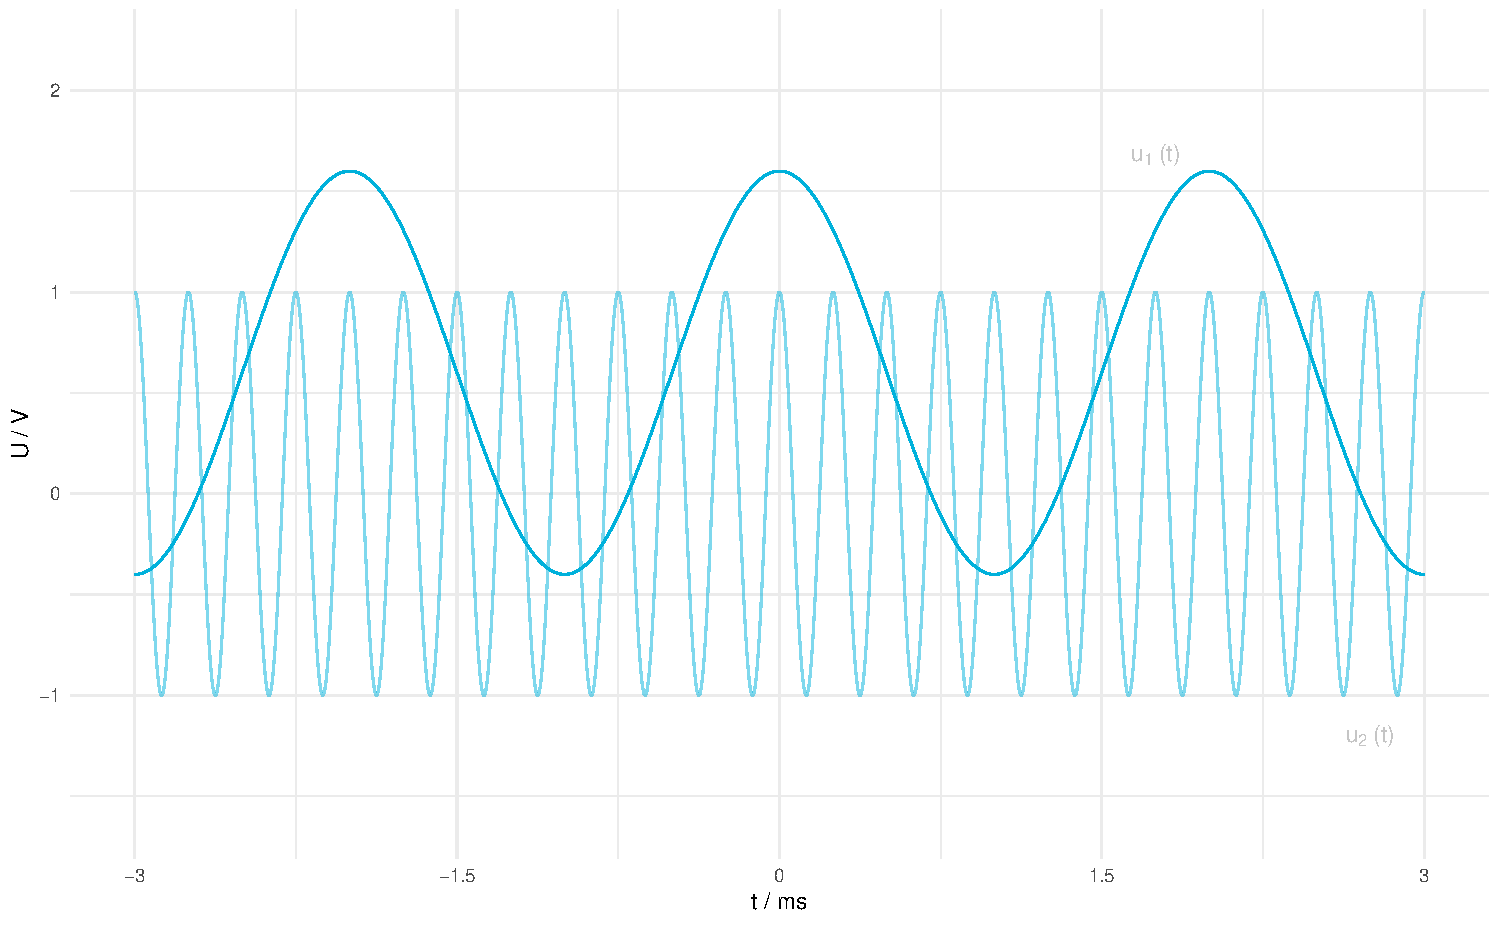
\includegraphics[width=\textwidth]{1_1/1_1_u1}
  \caption{$u_1(t)$ und $u_2(t)$}
\end{figure}

\begin{gather*}
  u_3(t) = u_1(t) \cdot u_2(t)\\
  = (U_0 + U_1 \cos{(\omega_1 t)}) \cdot U_2 \cos{(\omega_2 t)}\\
  = U_0 U_2 \cos{(\omega_2 t)} + U_1 U_2 [ \cos{(\omega_1 t)} \cdot \cos{(
    \omega_2 t)} ]\\
  \intertext{mithilfe der Gleichung aus "theoretische Grundlagen"\ ergibt
    sich}
  u_3(t)= U_0 \cos{(\omega_2 t)} + \frac{U_1 U_2}{2} \cdot \left[
    \cos{((\omega_1 - \omega_2)t)} + \cos{((\omega_1 + \omega_2) t)} \right]
\end{gather*}

\begin{figure}[H]
  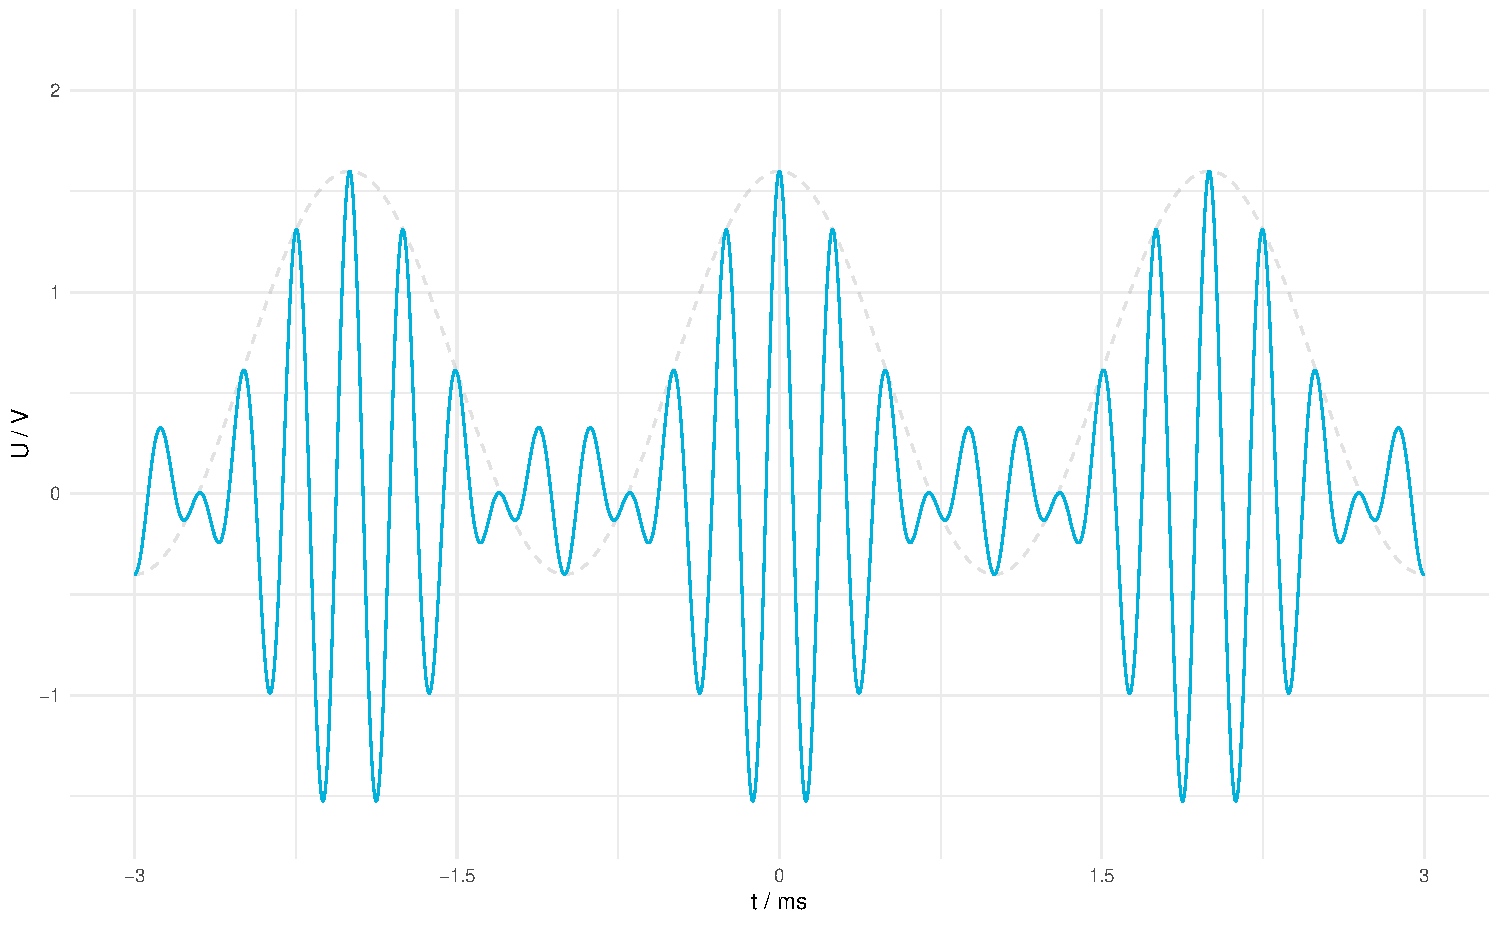
\includegraphics[width=\textwidth]{1_1/1_1_u3}
  \caption{$u_3(t)$; $u_1(t)$ ist als einhüllende Funktion erkennbar}
\end{figure}

\begin{gather}
	 \intertext{Fouriertransformation:}
U_3(\omega)= U_0 U_2 \cdot \mathcal{F}\{ \cos{(\omega_2 t)} \}+ \frac{U_1 U_2}{2} \cdot \left[
\mathcal{F}\{\cos{((\omega_1 - \omega_2)t)}\} +
\mathcal{F}\{\cos{((\omega_1+\omega_2) t)}\} \right] \nonumber
\intertext{mit}
%  \mathcal{F}\{ \cos{(2\pi f_0 t)} \} = \frac{1}{2} [ \delta{(f-f_0) + \delta{(f+f_0)}} ]
\mathcal{F}\{ \cos{(\omega_0 t)} \} = \frac{1}{2} [ \delta{(\omega-\omega_0) + \delta{(\omega+\omega_0)}} ] 
\intertext{ergibt sich}
	\begin{split}
	U_3(\omega) = \frac{U_0 U_2}{2}\cdot [ \delta(\omega-\omega_2) + \delta(\omega + \omega_2) ] \\ + \frac{U_1 U_2}{4} \cdot [ \delta(\omega-(\omega_1-\omega_2)) \\+ \delta(\omega + \omega_1-\omega_2) \\+ \delta(\omega-(\omega_1+\omega_2)) \\+ \delta(\omega + \omega_1 + \omega_2)]
	\end{split} \nonumber
\intertext{mit den vorgegebenen Werten:}
	\begin{split}
U_3(f) = 0.3 \cdot [ \delta(f-4\si{\kilo\hertz} + \delta(f + 4 \si{\kilo\hertz}) ] \\ + \frac{1}{4} \cdot [ \delta(f+3.5 \si{\kilo\hertz}) \\+ \delta(f - 3.5 \si{\kilo\hertz}) \\+ \delta(\omega-4.5 \si{\kilo\hertz}) \\+ \delta(\omega + 4.5 \si{\kilo\hertz})]
\end{split} \nonumber
\end{gather}

\begin{figure}[H]
  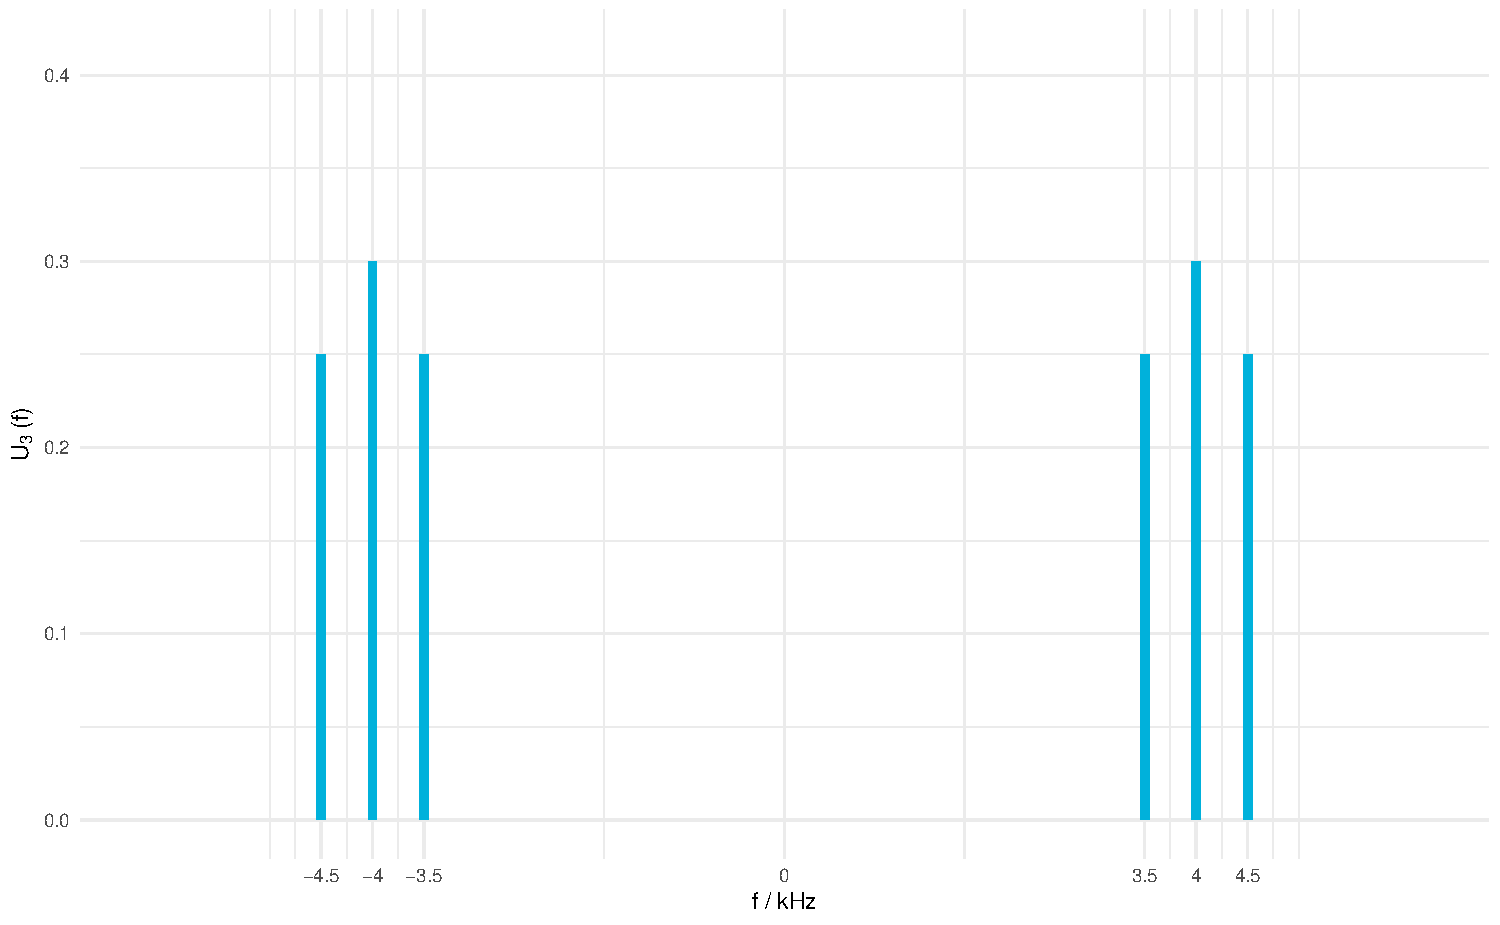
\includegraphics[width=\textwidth]{1_1/1_1_spektrum}
  \caption{Amplitudendichtespektrum von $u_3(t)$}
\end{figure}

%%%%%%%%%%%%%%%%%%%%%%%%%
\subsection{}

\begin{figure}[H]
  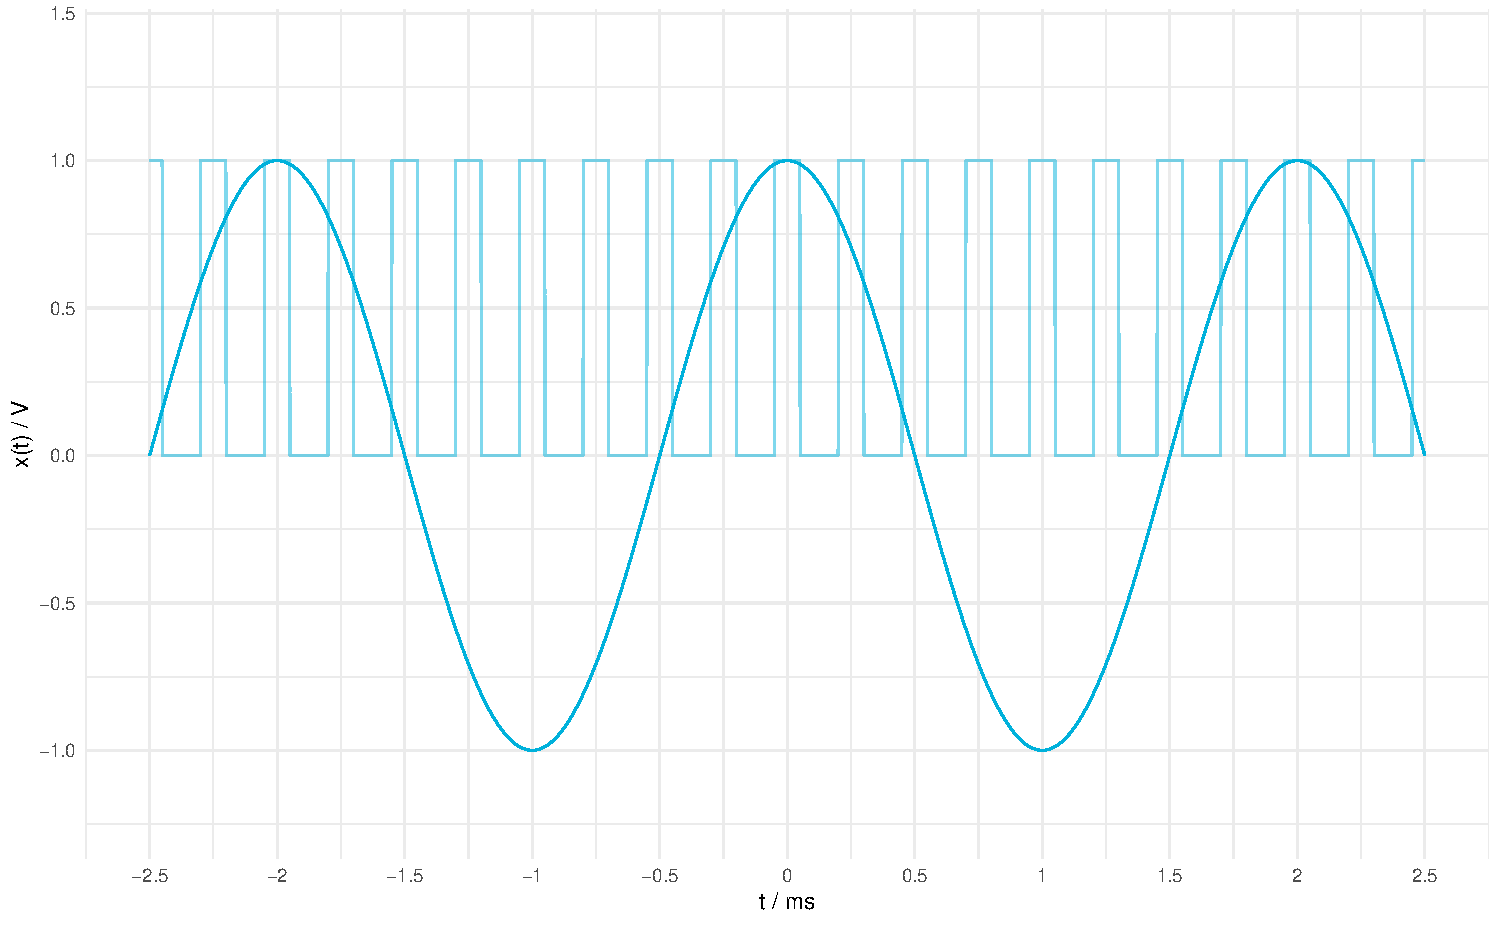
\includegraphics[width=\textwidth]{1_2/u1_carrier}
  \caption{$u_1(t)$ und $u_2(t)$}
\end{figure}

\begin{figure}[H]
  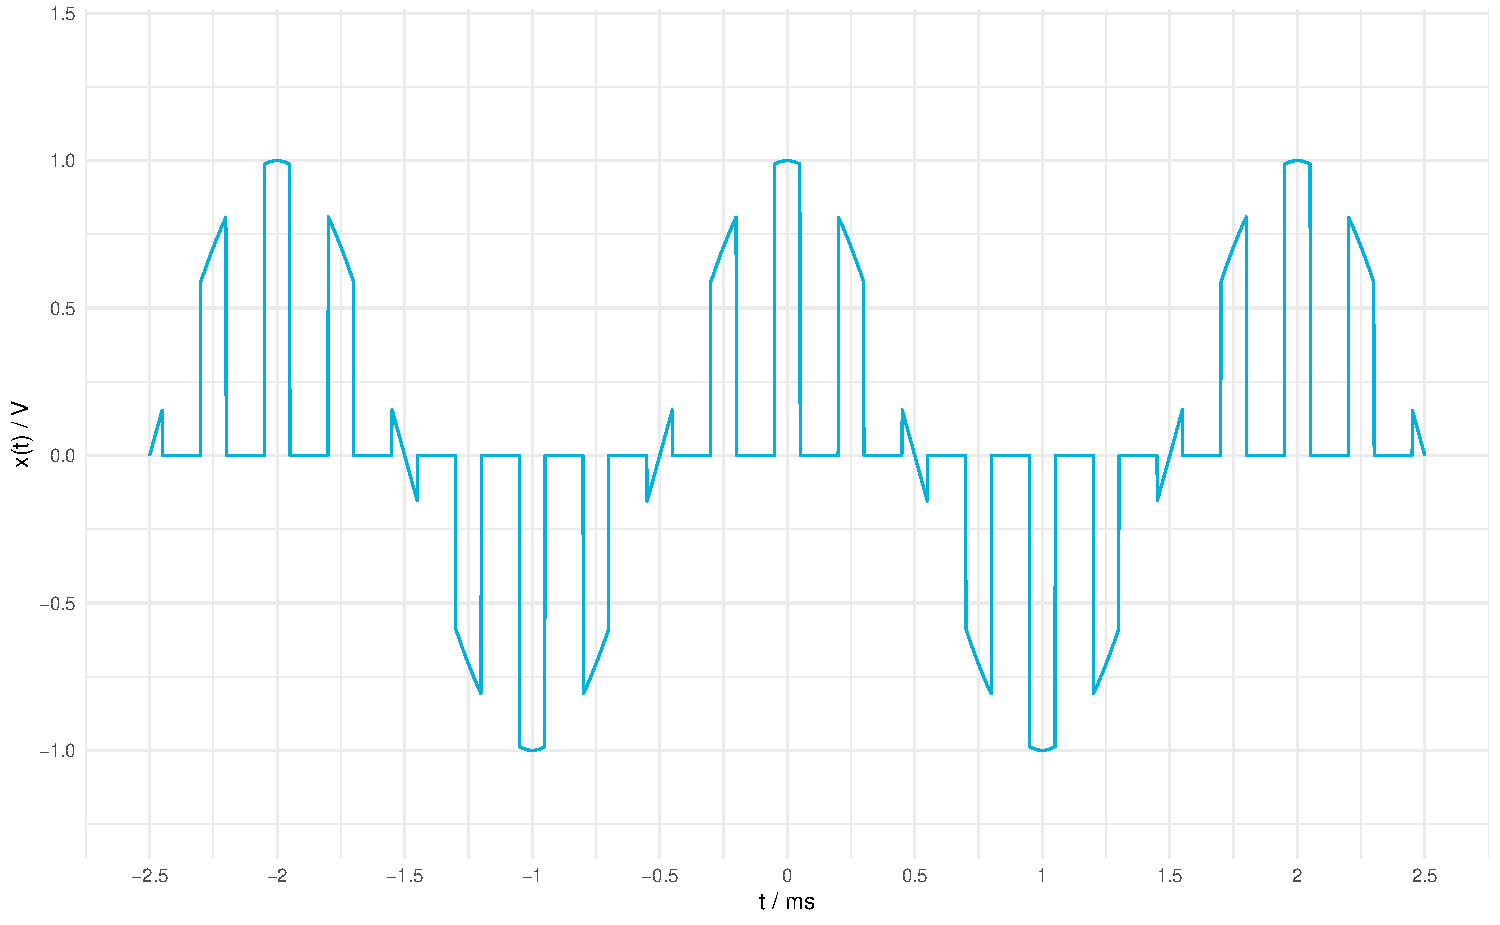
\includegraphics[width=\textwidth]{1_2/u3}
  \caption{$u_3(t)$ aus der Multiplikation von $u_1(t)$ mit dem Träger $u_2(t)$}
\end{figure}

\noindent Fouriertransformation:

Das Trägersignal $u_2(t)$ ist eine \emph{periodische} Rechteckfolge und hat
demnach ein \emph{diskretes} Spektrum, dessen Einhüllende die $\textrm{Si}$-Funktion
ist (Abbildung 6).

Die multiplikative Verknüpfung der Signale $u_1(t)$ und $u_2(t)$ im Zeitbereich
lässt sich in eine Faltung im Frequenzbereich überführen. Da dies analytisch nicht
so einfach ist, wird hier auf eine grafische Lösung zurückgegriffen. Dazu die Vorüberlegung:

\begin{gather*}
  X_3(f) = X_1(f) * X_2(f) \\
  X_2(f) = A \cdot \delta{(f-f_0)} \,\ \laplace \,\ {x_2(t) = A e^{j \cdot 2\pi \cdot f_0 \cdot t}}\\ 
  \intertext{(Verschiebungssatz)}
  X_3(f) = X_1(f) * A \cdot \delta{(f-f_0)} = A \cdot X_1(f - f_0)
\end{gather*}


\begin{figure}[H]
  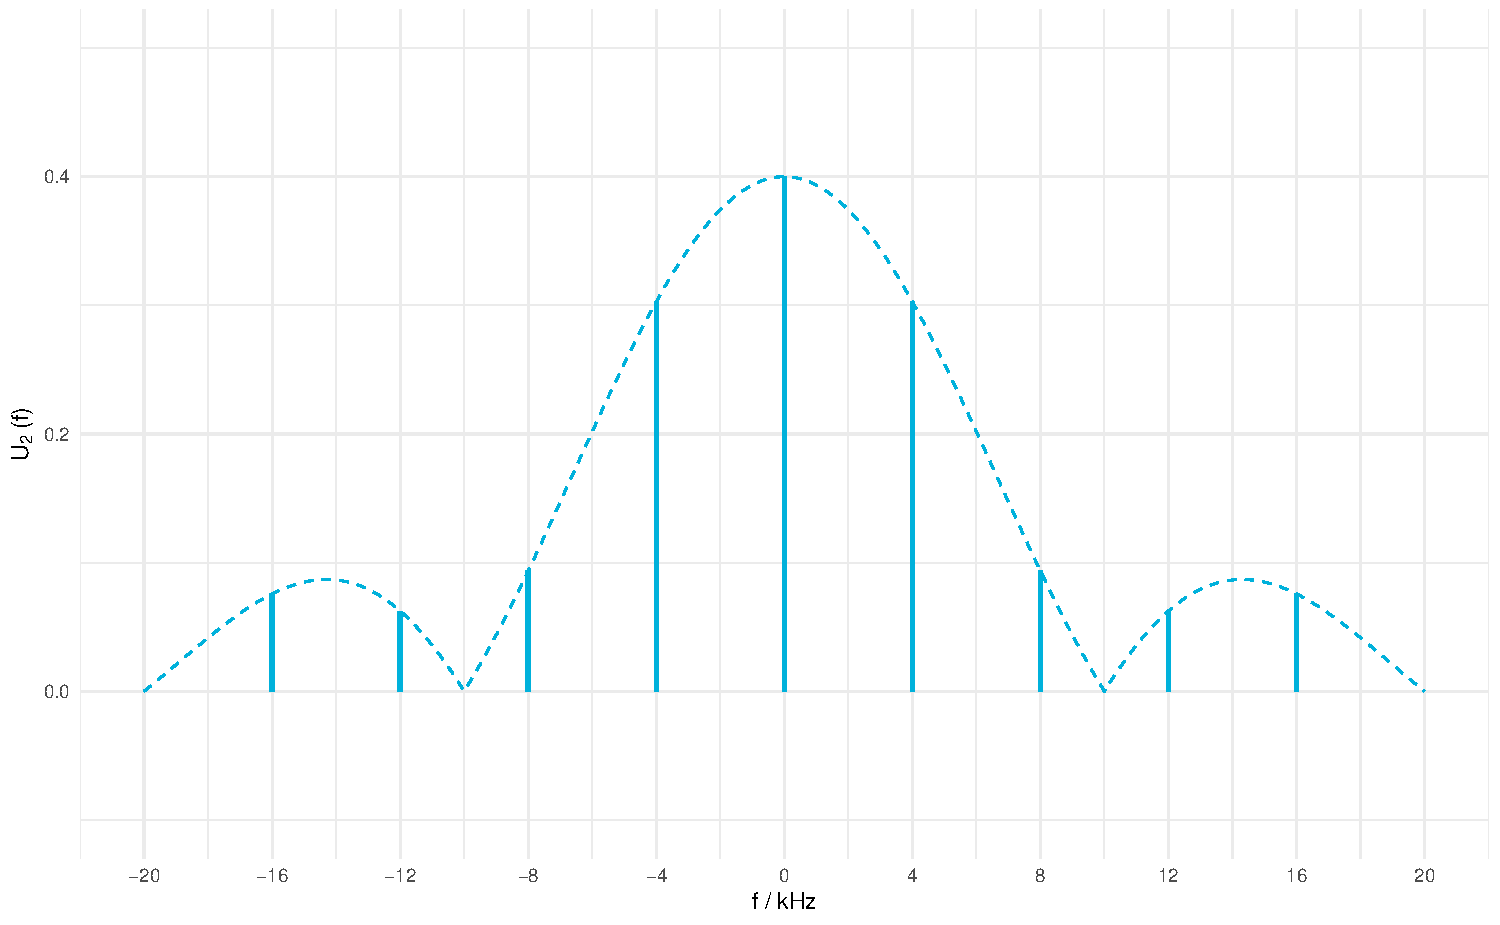
\includegraphics[width=\textwidth]{1_2/Si}
  \caption{Spektrum von $u_2(t)$, Einhüllende ist die Si-Funktion (Betrag) }
\end{figure}
 
Die einzelnen Spektrallinien des Rechtecksignals können in der Faltung beider
Funktionen im Frequenzbereich als Dirac-Impulse aufgefasst werden. Da diese sich
jeweils bei $n \cdot 4 \, \si{\kilo\hertz}$ wiederholen, wird die Transformation
des Nachrichtensignals (Gleichung 1) durch die Faltung um die Frequenz des Trägersignals
periodisch verschoben und mit der Amplitude der jeweiligen Träger-Impulse gewichtet.

\begin{figure}[H]
  \includegraphics[width=\textwidth]{1_2/Falti_mit_GA_träger_richtig}
  \caption{Resultierendes Amplitudenspektrum von $u_3(t)$ mit Gleichanteil im Träger}
\end{figure}

\begin{figure}[H]
  \includegraphics[width=\textwidth]{1_2/Falti_ohne_GA_träger_richtig}
  \caption{Resultierendes Amplitudenspektrum von $u_3(t)$ ohne Gleichanteil im Träger}
\end{figure}

\begin{figure}[H]
  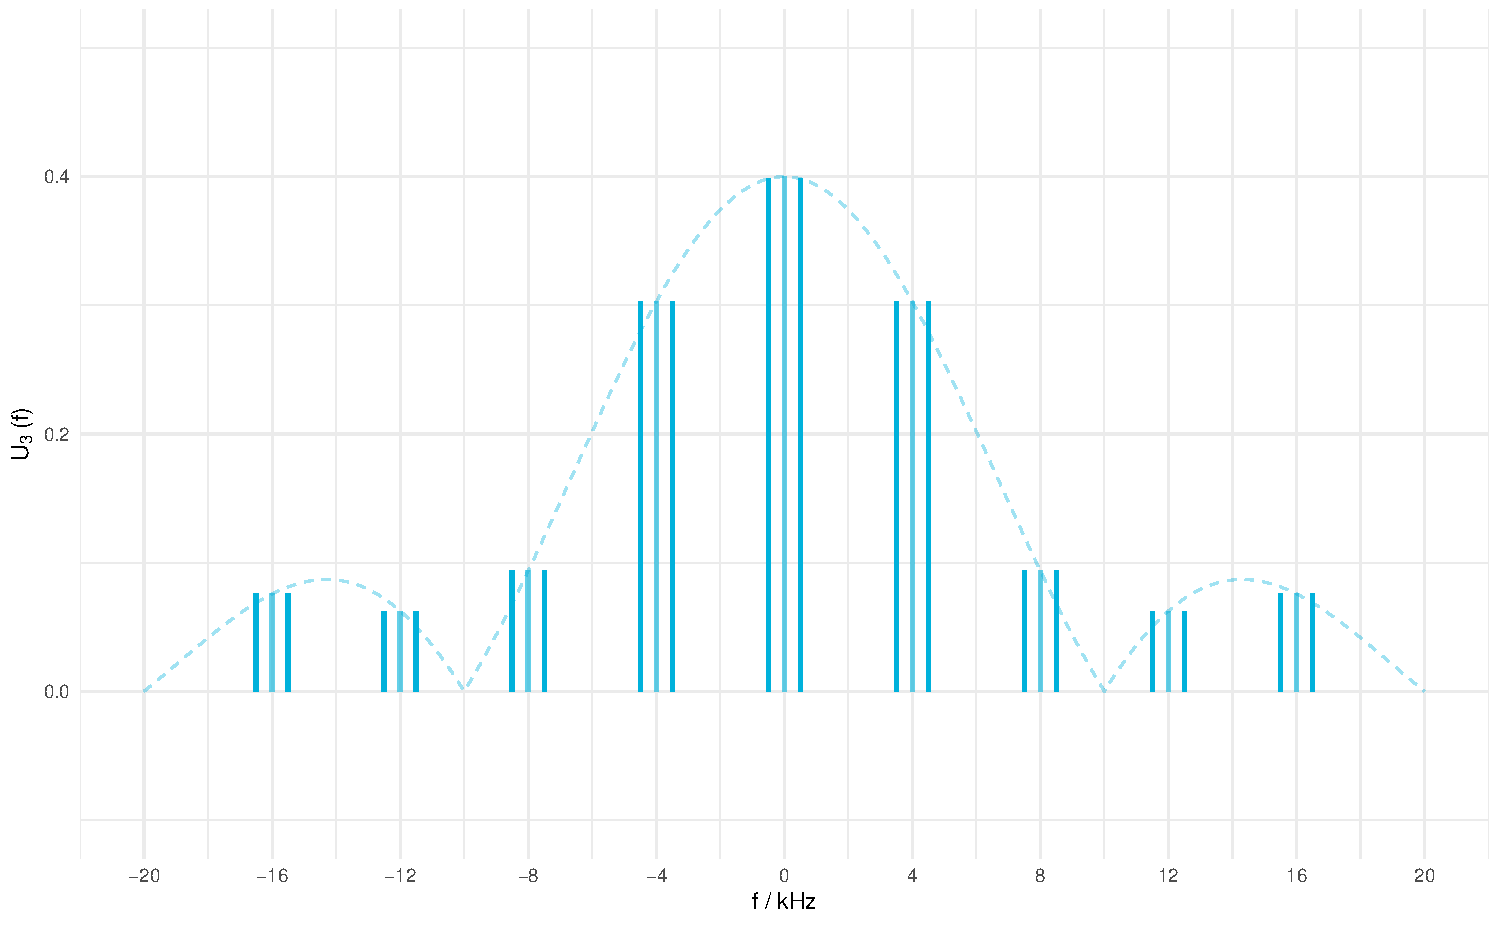
\includegraphics[width=\textwidth]{1_2/Falti_mit_GA_nachricht_richtig}
  \caption{Resultierendes Amplitudenspektrum von $u_3(t)$ mit Gleichanteil in
    Träger und Nachrichtensignal}
\end{figure}

\subsection{Praktische Anwendungsmöglichkeiten}

Die Multiplikation von Zeitsignalen findet Anwendung in der Nachrichtenübertragung. Dort kann das zu übertragene Signal mit einem \emph{Trägersignal} multipliziert werden, um zum Einen das Signal in einen für die Antennentechnik brauchbaren\footnote{Änderung der Übertragungseigenschaften des Signals mit der Frequenz} Frequenzbereich zu bringen und zum Anderen das Signal am Empfänger von anderen Signalen in der Frequenz unterscheiden zu können (vgl. 1.1).

Außerdem nutzen Oszilloskope die Multiplikation mit einem Rechtecksignal um ein Fenster des aufgenommenen Signals zu erhalten, welches dann fourieranalysiert werden kann.

\section{Versuchsaufgaben}

\subsection{}

\begin{figure}[H]
  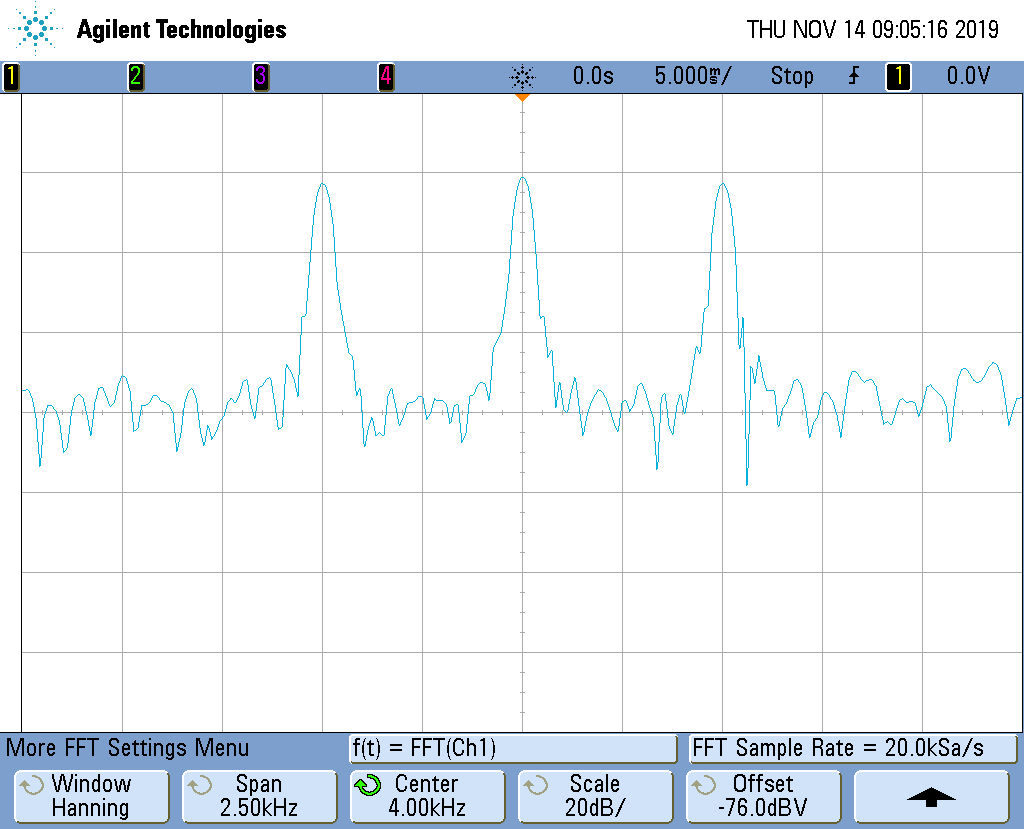
\includegraphics[width=\textwidth]{2_1/scope_5_blue}
  \caption{FFT von $u_3(t)$ analog Aufgabe 1}
\end{figure}

Wie in Abbildung 10 zu sehen, stimmen die ermittelten Frequenzen mit denen der
Vorbereitungsaufgabe überein.
Durch Limitierungen des Oszilloskops (z.B.
Fensterung) und der Soundkarte sowie Störeinflüsse sieht man keine exakt
diskreten Amplitudenlinien, die Maxima sind jedoch klar bei den berechneten
Frequenzen erkennbar.

\begin{figure}[H]
  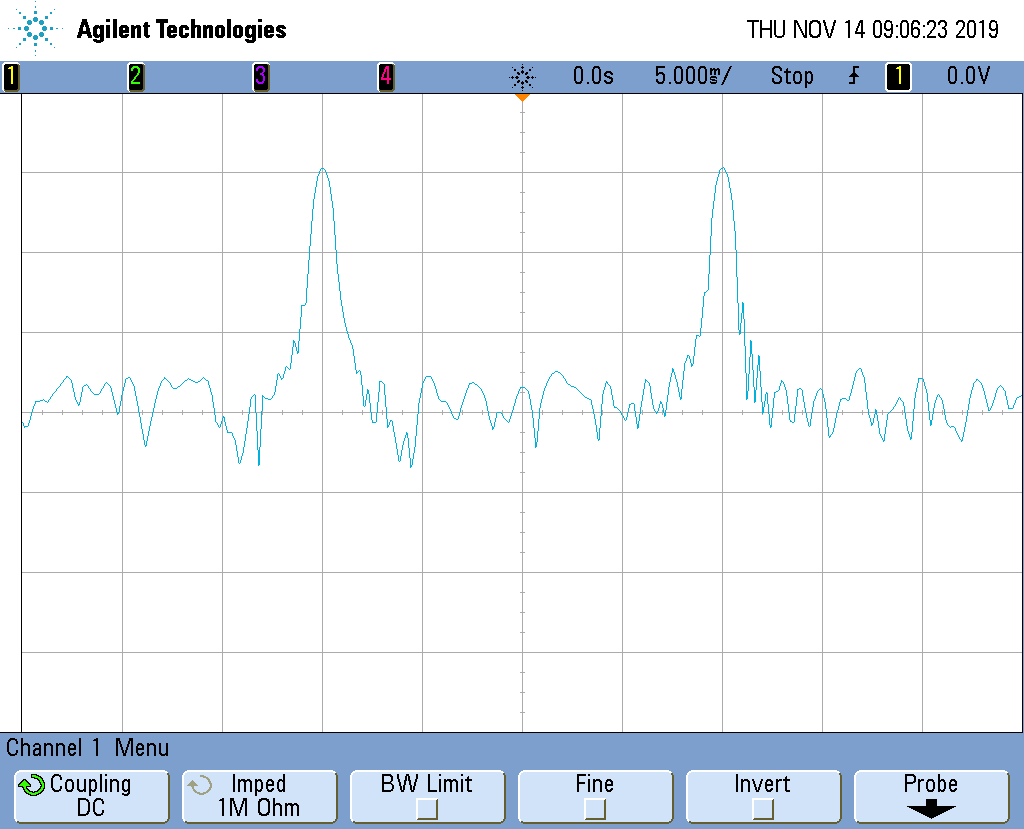
\includegraphics[width=\textwidth]{2_1/scope_6_blue}
  \caption{FFT von $u_3(t)$ ohne Gleichanteil der Nachricht}
\end{figure}

Nach Entfernen des Gleichanteils des Nachrichtensignals verschwindet die Frequenz des
Träges aus dem Betragsspektrum des übertragenen Signals (Abbildung 11). Der Gleichanteil der Nachricht lässt also den Träger erscheinen. 

\begin{figure}[H]
  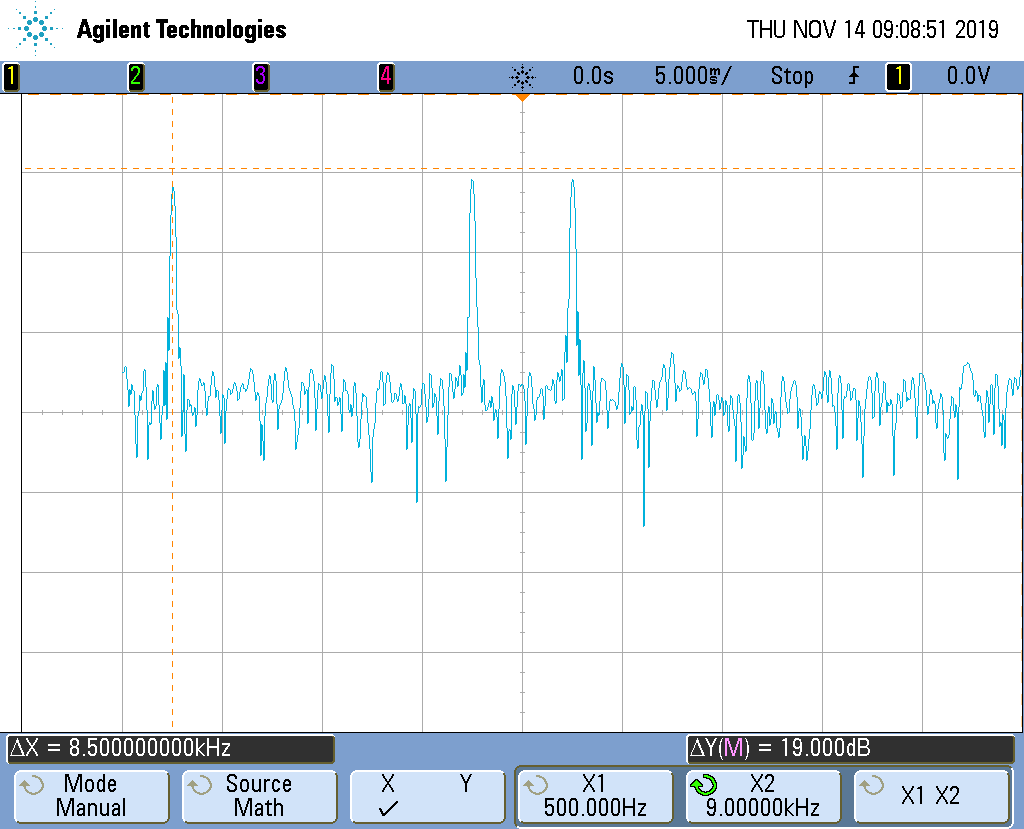
\includegraphics[width=\textwidth]{2_1/scope_7_blue}
  \caption{FFT von $u_3(t)$ mit Gleichanteil im Träger}
\end{figure}

Wird nun das Trägersignal mit einem Gleichanteil versehen, wird die Originalfrequenz des Nachrichtensignals mitübertragen. Der Gleichanteil des Trägersignals lässt die Frequenz(en) des Nachrichtensignals erscheinen.

Erhöht man jetzt die Frequenz des Nachrichtensignals, rücken diese und die
untere Frequenz des ursprünglich gefalteten Signals immer näher zusammen (Abbildung 13). Die beiden ursprünglichen Frequenzen rücken dabei weiter auseinander. Bei einer Frequenz von $2 \,\ \si{\kilo\hertz}$ überlappen sich die Originalfrequenz und die ursprüngliche Faltungsfrequenz und sind nicht mehr unterscheidbar.

\begin{figure}[H]
  \begin{center}
  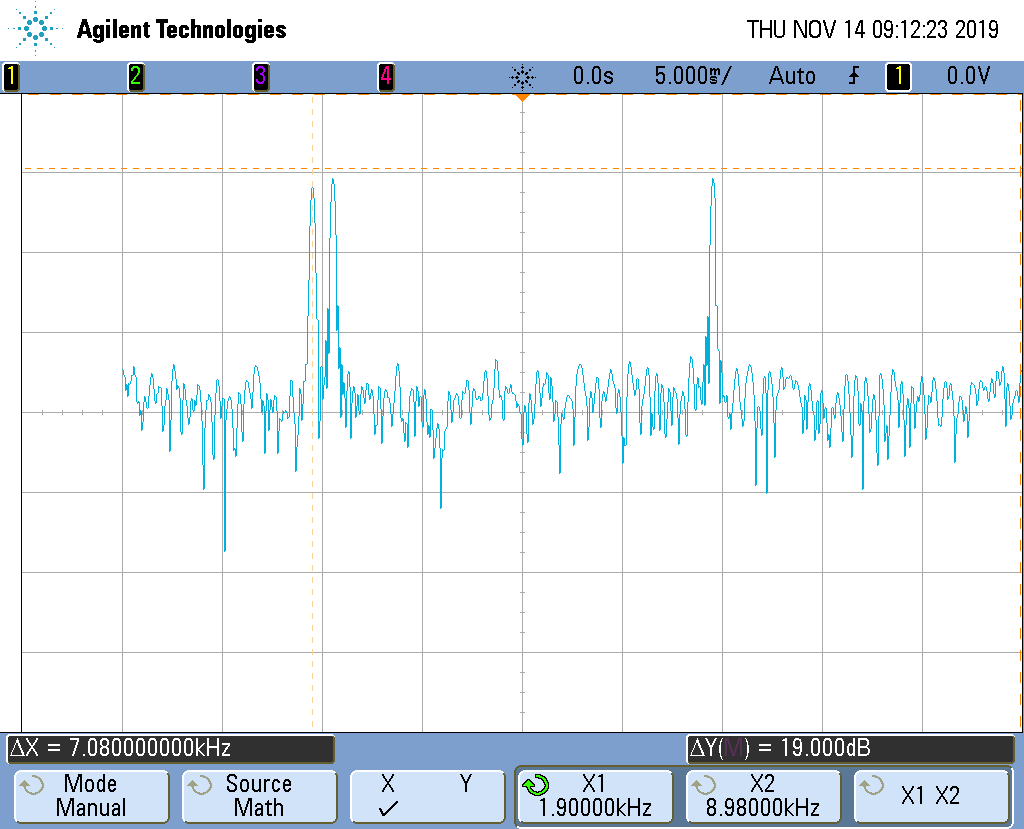
\includegraphics[height=0.618\textwidth]{2_1/scope_9_blue}
  \caption{Frequenzen nahe der Überschneidung}
  \end{center}
\end{figure}

\begin{figure}[H]
  \begin{center}
  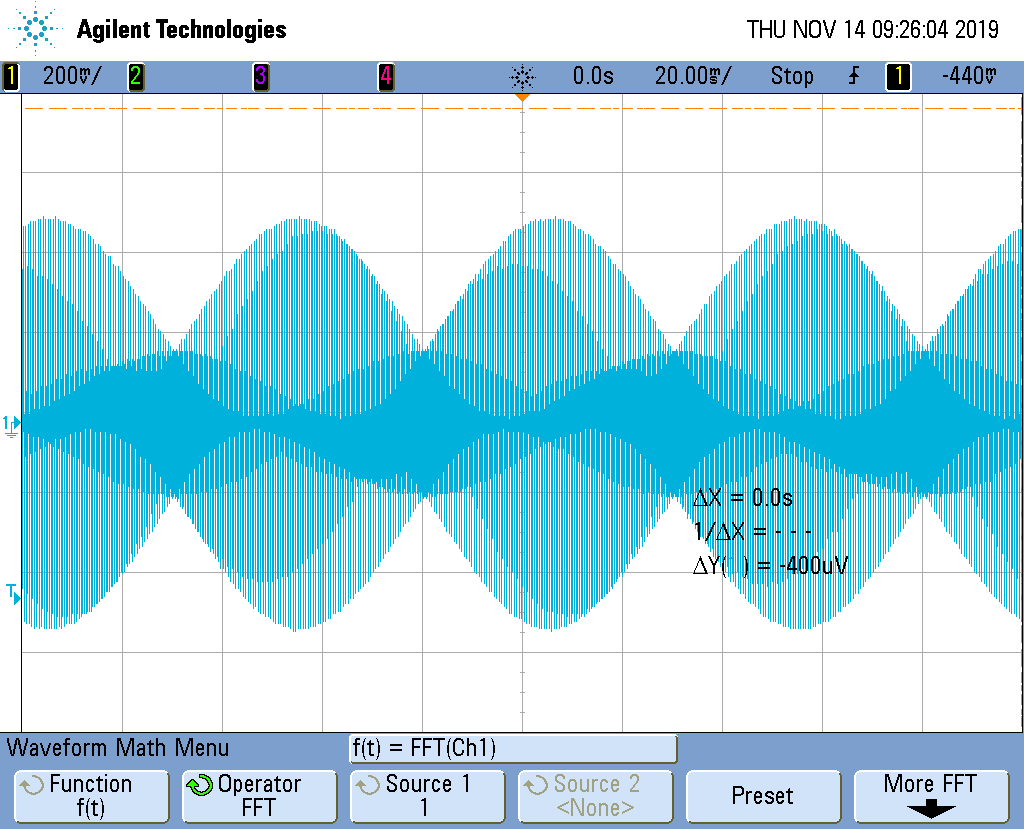
\includegraphics[height=0.618\textwidth]{2_1/scope_10_blue}
  \caption{Zeitsignal bei Annäherung der Frequenzen von $u_1(t)$ und $u_3(t)$}
  \end{center}
\end{figure}

Bei Frequenzen, die sehr nahe an der Überschneidungsfrequenz sind (z.B. $1990
\,\ \si{\hertz}$), entstehen Schwebungen im Zeitbereich (Abbildung 14).


\subsection{}

\begin{figure}[H]
	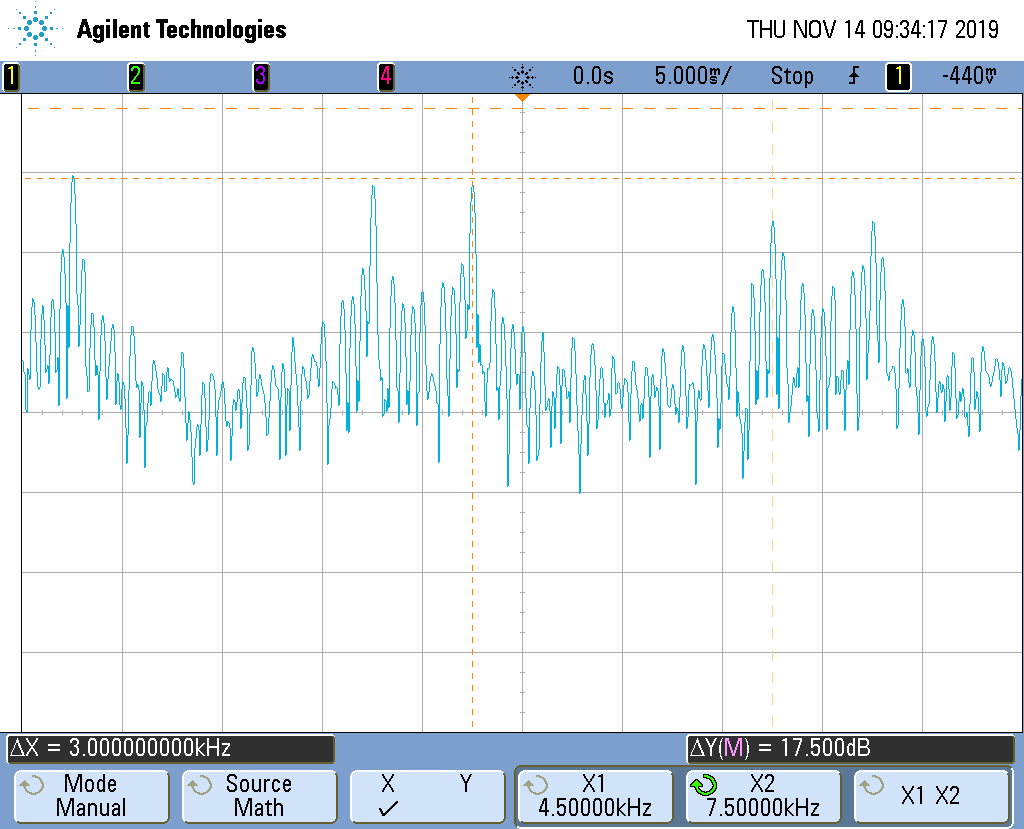
\includegraphics[width=\textwidth]{2_2/scope_11_blue}
	\caption{FFT von $u_3(t)$ analog Aufgabe 2}
\end{figure}

Wie in Abbildung 15 zu sehen, stimmen die ermittelten Frequenzen mit denen der Vorbereitungsaufgabe überein. 

\begin{figure}[H]
\begin{center}
	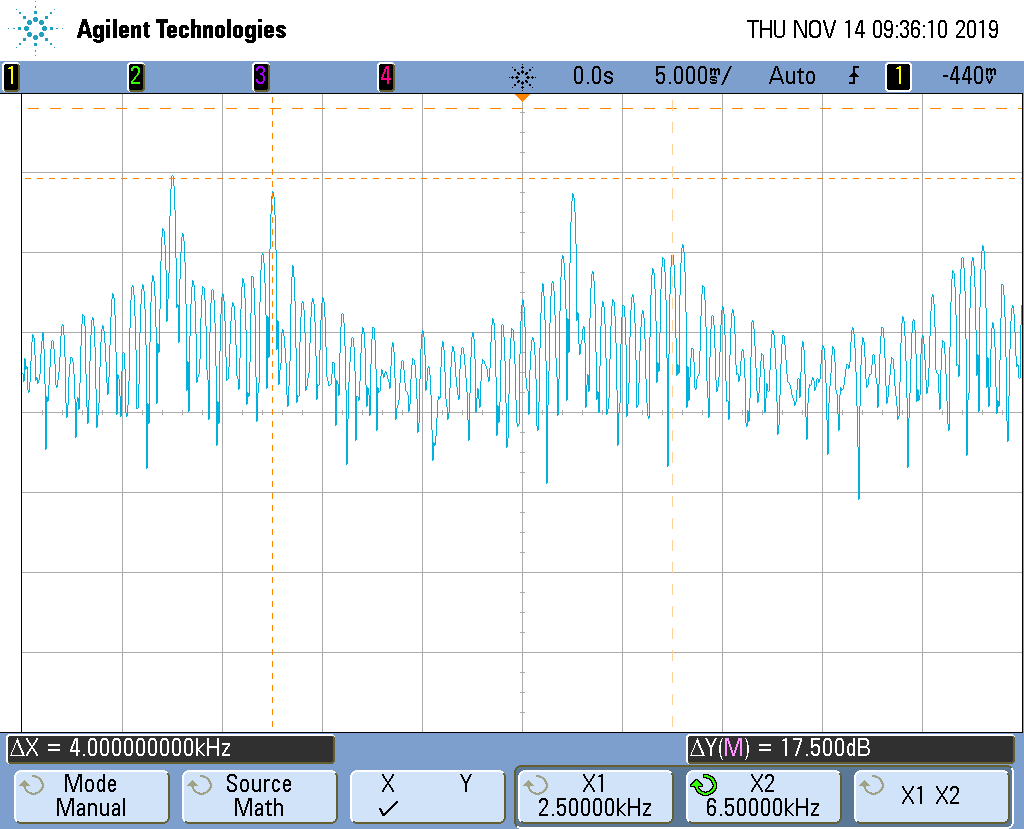
\includegraphics[height=0.618\textwidth]{2_2/scope_12_blue}
	\caption{Bewegung der Frequenzanteile durch Variation der Nachrichtenfrequenz, noch keine Überschneidung}
\end{center}
\end{figure}
\begin{figure}[H]
\begin{center}
	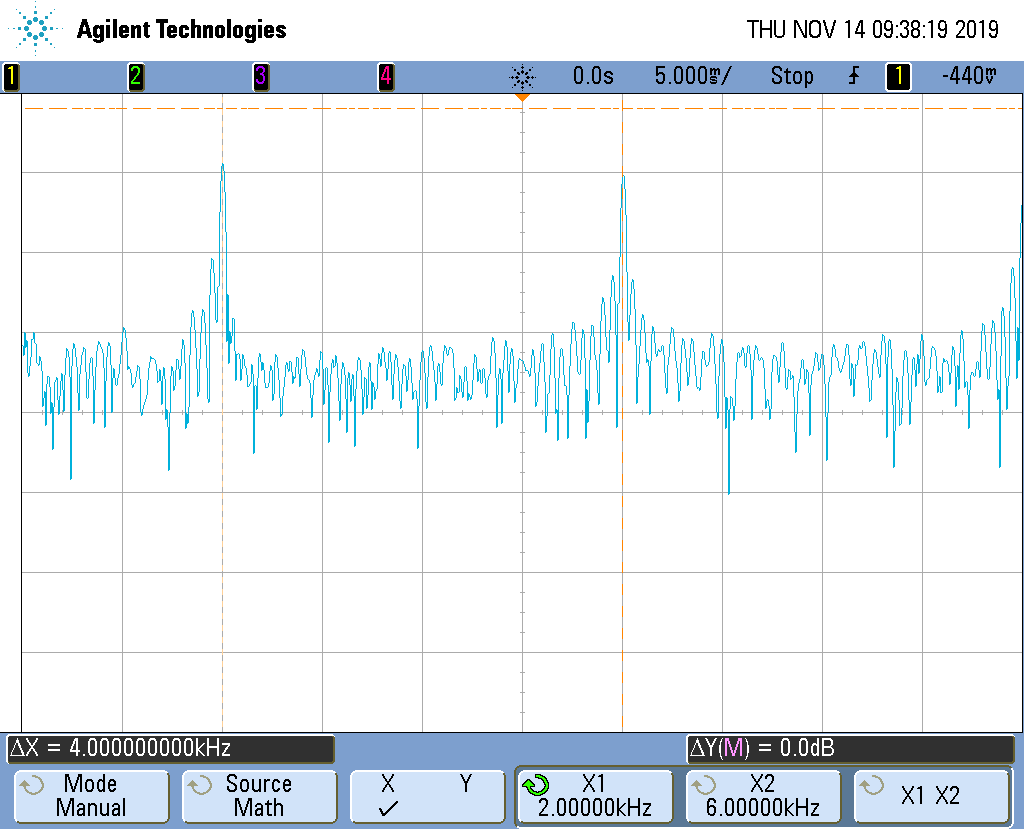
\includegraphics[height=0.618\textwidth]{2_2/scope_14_blue}
	\caption{Bewegung der Frequenzanteile, Überschneidung bei $2 \, \si{\kilo\hertz}$}
\end{center}
\end{figure}

Bei Frequenzerhöhung weichen, wie auch in Versuchsaufgabe 2.1, die Frequenzen um
das Trägerzentrum auseinander bis sie sich mit anderen bei (z.B.) $2 \,\
\si{\kilo\hertz}$ treffen (Abblidung 16).

Die periodisch auftretenden Frequenzbreiten um $n \cdot 4 \, \si{\kilo\hertz}$ können z.B. als Sender bei
einer bestimmten Trägerfrequenz aufgefasst werden, welche zudem eine bestimmte
Bandbreite für die zu übertragenden Nachrichtensignale benötigen ($U_1(f)$). Die in
Versuchsaufgabe 1 und 2 dargestellte Problematik der Überlappung von
Frequenzanteilen zeigt, dass in der Praxis ein minimaler Frequenzabstand zwischen zwei
Sendern notwendig ist, da sonst kein Filter realisierbar wäre, das es ermöglicht,
die einzelnen Signale in der Frequenz unterscheiden zu können. 

\begin{figure}[H]
\begin{center}
	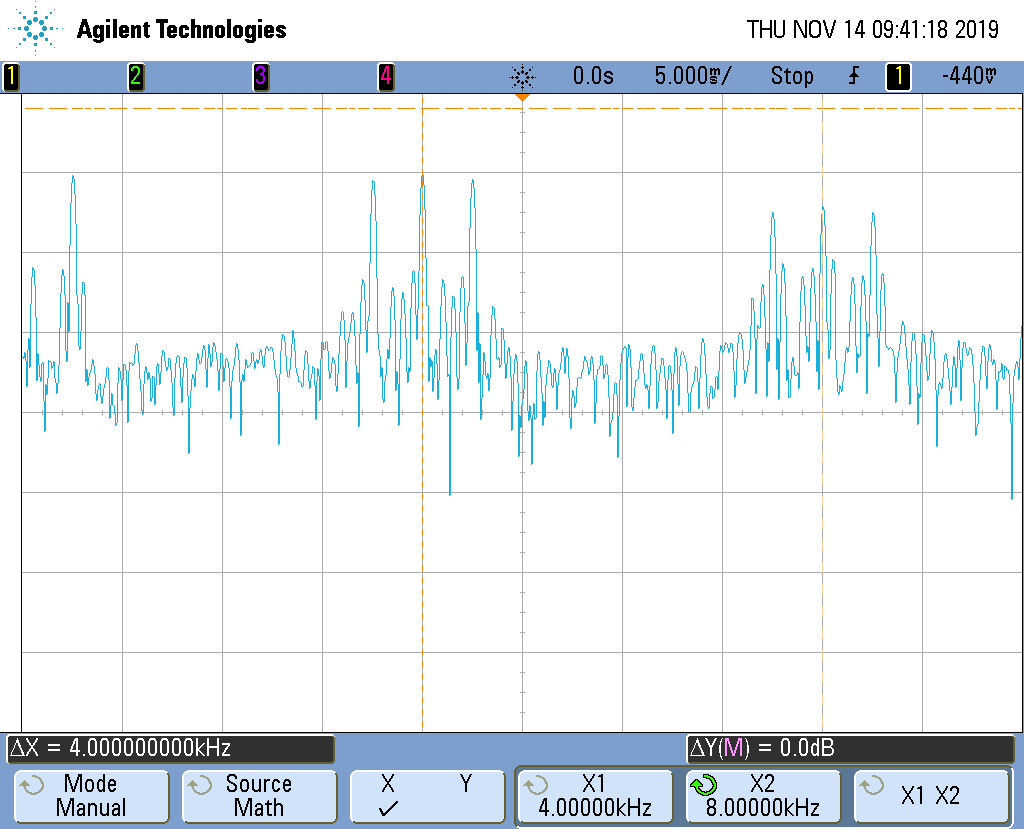
\includegraphics[width=\textwidth]{2_2/scope_15_blue}
	\caption{FFT von $u_3(t)$ mit Gleichanteil in der Nachricht}
\end{center}
\end{figure}

\begin{figure}[H]
\begin{center}
	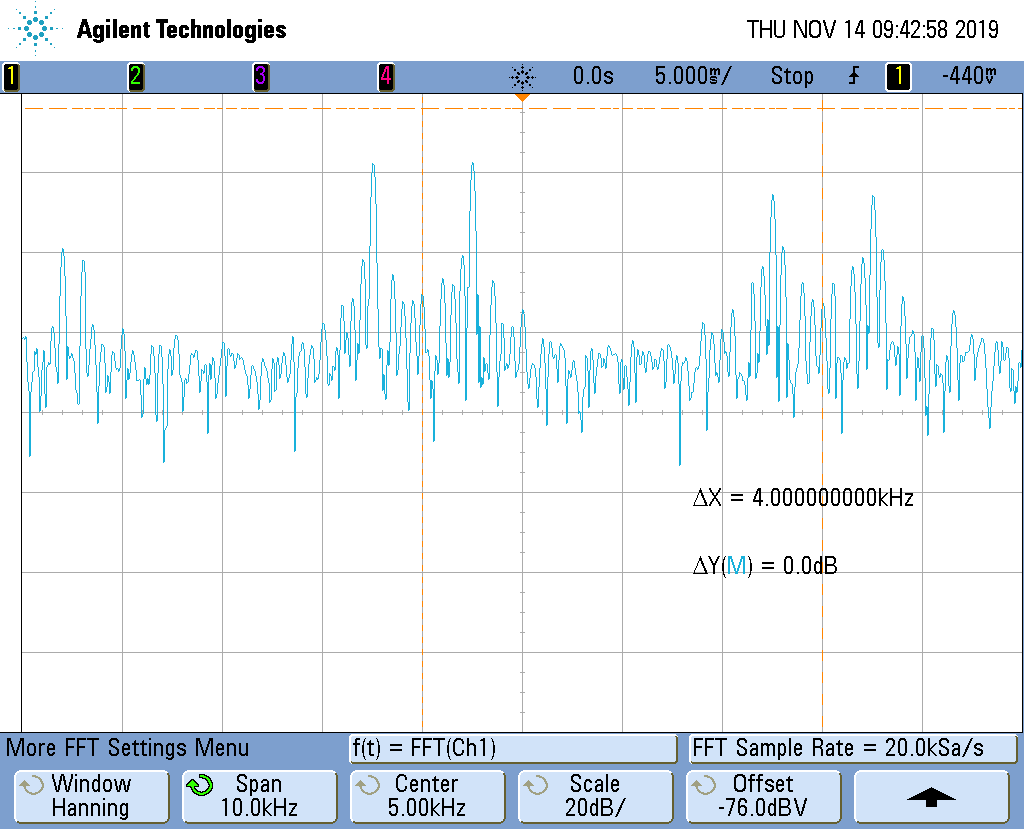
\includegraphics[width=\textwidth]{2_2/scope_16_blue}
	\caption{FFT von $u_3(t)$ ohne Gleichanteil in der Nachricht}
  \end{center}
\end{figure}
Wie auch in der Versuchsaufgabe 2.1 lässt ein hinzugefügter Gleichanteil im
Träger- bzw. Nachrichtensignal die Originalfrequenz des jeweils anderen Signals
im Spektrum erscheinen (Abbildung 18 und 19).


\end{document}
